\documentclass[11pt]{article}

\usepackage[margin=1in]{geometry}
\usepackage{amsmath,amssymb,amsthm}
\usepackage{hyperref}
\usepackage{enumitem}
\usepackage{graphicx}
\usepackage{xcolor}
\usepackage{listings}
\usepackage{booktabs}

\newtheorem{theorem}{Theorem}
\newtheorem{proposition}[theorem]{Proposition}
\newtheorem{corollary}[theorem]{Corollary}
\newtheorem*{openproblem}{Open Problem}

\lstset{
    basicstyle=\ttfamily\small,
    keywordstyle=\color{blue!60!black},
    commentstyle=\color{gray},
    stringstyle=\color{orange!70!black},
    breaklines=true,
    columns=fullflexible,
    frame=single,
    xleftmargin=1em,
    xrightmargin=1em,
}

\title{Critical Temperature and Strict-Saddle Instability of the Splay State in Self-Attention Dynamics}
\author{}
\date{}

\begin{document}
\maketitle

\begin{abstract}
We study the linear stability of the maximally dispersed (``splay'') configuration in a family of similarity-coupled interacting particle systems on the sphere, with coupling strength set by an inverse temperature $\beta$. Such systems arise as a mean-field, continuous-depth model of self-attention, the core mechanism of Transformer neural networks, in which particle clustering corresponds to collapse of token representations. On the circle ($d=2$), Geshkovski, Letrouit, Polyanskiy \& Rigollet (\emph{A Mathematical Perspective on Transformers}, Bull.\ AMS 2025) pose as an open problem whether every critical point other than the global energy maximum is a strict saddle for the associated gradient flow. We resolve this exactly for the splay state, combining the classical Bessel-function expansion of the coupling kernel with the circulant structure its cyclic symmetry imposes on the stability matrix. This yields a closed-form Jacobian eigenvalue at every mode, two exact special cases obtained by hand ($n=2$: decay as $e^{-\beta}$; $n=4$: unbounded growth, exactly $\beta$), and numerically robust strict-saddle instability at every finite $\beta$ tested, $n=2,\dots,8$. An exact bridge to the true, softmax-normalized dynamics then proves the real system's instability rate vanishes as $\beta\to\infty$ for every $n$: the splay state freezes rather than further destabilizes at low temperature, the opposite of what the unbounded surrogate rate alone would suggest. This bridge yields two falsifiable definitions of an operational critical temperature: a closed-form finite-depth crossover $\beta_c(n,L)$, and a finite-noise order/disorder transition $\beta_c(n,D)$ located empirically via two independent order parameters --- the participation ratio and the classical Kuramoto synchronization parameter --- that cross coherently and sharpen under increased sampling. Three extensions test the robustness of the low-temperature freezing mechanism. On $\mathbb{S}^{d-1}$, the regular simplex ($d=3,\dots,9$) generalizes the splay state, is an exact equilibrium by symmetry, and remains numerically a strict saddle with a clean two-eigenvalue structure. Under causal masking, the transition is solved exactly for $n=2$ (the noncausal rate exactly halved), and the same $\beta\to\infty$ vanishing persists numerically to $n=8$ despite the splay state no longer being an exact equilibrium. Adding a token-wise feed-forward nonlinearity breaks the mechanism entirely: since the feed-forward term carries no $\beta$-dependence, the instability rate instead saturates at a nonzero constant fixed by the feed-forward layer's own Jacobian, showing the freezing is specific to the similarity-coupling term rather than the full network layer.
\end{abstract}

\noindent\textbf{Keywords:} synchronization and the Kuramoto model; strict saddle points; critical (inverse) temperature; order--disorder phase transition; interacting particle systems; Bessel functions and circulant matrices; self-attention dynamics; Transformers

\section{Introduction}
\label{sec:intro}

Self-attention is the mechanism that lets a Transformer (Vaswani et al., 2017) mix information across tokens at every layer, and it is essentially the entire computational novelty behind large language models: everything else in the architecture (feed-forward blocks, normalization, residual connections) is generic deep-learning machinery also found in non-sequence models. A substantial body of empirical work on deep Transformers has documented that token representations tend to become increasingly similar to one another as depth increases --- variously described as \emph{oversmoothing}, \emph{token uniformity}, \emph{representation collapse}, or \emph{(attention-)rank collapse} (Dong, Cordonnier \& Loukas, 2021; Noci et al., 2022) --- and that this collapse can degrade a model's effective capacity, since near-identical token embeddings carry little information for downstream layers, attention heads, or the unembedding layer to act on. This is exactly the phenomenon the interacting-particle-system viewpoint below makes mathematically precise: with the feed-forward and normalization sublayers stripped away, pure self-attention is \emph{exactly} a dynamical system on a sphere whose only free parameter is an inverse-temperature $\beta$ (set, in a real model, by the scale of the learned query/key weights together with the usual $1/\sqrt{d_k}$ logit scaling), and whose generic long-time behavior is provably clustering. Understanding how fast that clustering sets in as a function of $\beta$ --- and whether there is a sharp scale $\beta_c$ separating ``still doing useful, information-preserving mixing'' from ``already collapsing tokens together'' --- is therefore a first-principles handle on a purely empirical, architecture-level question, and is the object of study of this paper.

The interacting-particle-system picture of self-attention (Geshkovski, Letrouit, Polyanskiy \& Rigollet, 2023, henceforth GLPR23; surveyed comprehensively in Geshkovski, Letrouit, Polyanskiy \& Rigollet, 2025, henceforth the \emph{Survey}) treats token embeddings across depth as particles on a sphere $\mathbb{S}^{d-1}$, evolving under a self-attention drift with $Q=K=V=I$:
\begin{equation}
    \dot X_t^i = \frac{1}{Z^i(t)} \sum_{j=1}^n e^{\beta \langle X_t^i,\, X_t^j\rangle}\, X_t^j - X_t^i\Big\langle X_t^i, \frac{1}{Z^i(t)} \sum_{j=1}^n e^{\beta \langle X_t^i,\, X_t^j\rangle}\, X_t^j\Big\rangle,
    \qquad Z^i(t) = \sum_{j=1}^n e^{\beta \langle X_t^i,\, X_t^j\rangle},
    \label{eq:sa}
\end{equation}
the tangential projection of a softmax-weighted average onto the sphere, with $\beta>0$ an inverse-temperature parameter absorbing the usual query/key logit scale. The softmax weight attached to token $j$ in token $i$'s update, $e^{\beta\langle X^i,X^j\rangle}/Z^i(t)$, is by construction an increasing function of how similar $X^i$ and $X^j$ already are, so each token's update pulls it toward whichever other tokens it already resembles most. This is a positive-feedback, ``rich-get-richer'' coupling --- formally the same kind of similarity-weighted attraction that drives synchronization in the Kuramoto model of coupled oscillators (Kuramoto, 1975; Strogatz, 2000; Acebrón, Bonilla, P\'erez Vicente, Ritort \& Spigler, 2005), or consensus in flocking and opinion-dynamics models (Vicsek, Czir\'ok, Ben-Jacob, Cohen \& Shochet, 1995; Cucker \& Smale, 2007; Hegselmann \& Krause, 2002) --- and it is \emph{why} self-attention clusters tokens at all: once two tokens are even slightly more aligned than average, they attend to each other more strongly than to the rest, move closer together, attend even more strongly next step, and so on, with nothing in the noiseless dynamics to arrest the reinforcement once it starts. GLPR23 and its follow-ups make this rigorous, proving that under \eqref{eq:sa}, tokens provably cluster into a small number of leader groups as $t\to\infty$, for essentially any $\beta>0$ and general $Q,K$ pairs on the sphere.

Real Transformers have $\beta$ set (and shaped by training) rather than externally fixed: it is controlled jointly by the norm of the learned query/key projections and the conventional $1/\sqrt{d_k}$ scaling, and it can differ substantially across layers and heads of the same trained model. We take $\beta_c$ to denote, informally, the \emph{critical inverse temperature} at which the qualitative character of the token dynamics changes: below $\beta_c$, attention stays diffuse enough that a maximally spread-out configuration of tokens is dynamically stable, or destabilizes only slowly, while above $\beta_c$ attention concentrates sharply enough on each token's closest neighbors that dispersal becomes strongly unstable and the tokens collapse toward one or a few clusters within a handful of layers. \S\ref{sec:substitutes} makes two versions of $\beta_c$ precise and computable: a finite-depth crossover $\beta_c(n,L)$, the value of $\beta$ at which the splay state's instability rate first exceeds what $L$ layers can amplify into visible clustering, and a finite-noise order/disorder threshold $\beta_c(n,D)$, the value of $\beta$ at which a genuine bifurcation moves the system's long-run statistics from a disordered plateau to a clustered one. Knowing $\beta_c$ matters because it turns a qualitative worry --- is a given layer smoothing away useful information? --- into a quantitative, checkable diagnostic: a layer whose effective $\beta_\ell$ sits well below $\beta_c$ is, in this idealized model, still doing genuine, slowly-mixing work; $\beta_\ell\gg\beta_c$ signals a layer already deep in the frozen, oversmoothing regime; and $\beta_\ell\approx\beta_c$ marks the boundary where a small change in scale --- from further training, or from a change in input norm --- can qualitatively change what the layer does. A natural diagnostic question follows: is a given layer's effective $\beta_\ell$ near $\beta_c$? Answering it requires actually knowing $\beta_c$ for some tractable reference system, which is what this paper provides.

A \emph{bifurcation}, in the dynamical-systems sense used throughout this paper, is a qualitative change in the number or stability of a system's equilibria as a control parameter --- here $\beta$ --- crosses a threshold; the textbook example is the \emph{pitchfork bifurcation}, in which a single stable equilibrium loses stability at a critical parameter value and splits into two new stable equilibria on either side of it. It is natural to guess that self-attention exhibits exactly this kind of transition: at $\beta=0$ attention is uniform and the maximally dispersed configuration is at worst marginally stable, as in the classical, zero-coupling Kuramoto model, so dispersal might remain a genuine local attractor up to some threshold $\beta_c$, beyond which the sharpening softmax finally destabilizes it and triggers collapse. One of this paper's central findings is that this naive picture is \emph{wrong} for the idealized, noiseless dynamics \eqref{eq:sa}--\eqref{eq:usa} below: the maximally dispersed ``splay'' configuration turns out to already be unstable at \emph{every} $\beta>0$, so there is no finite bifurcation threshold at all in that regime --- increasing $\beta$ only changes \emph{how fast} the instability acts (in real self-attention, ever more slowly, Corollary~\ref{cor:always-vanishes}), never whether it acts. A genuine bifurcation in $\beta$ only reappears once this idealization is relaxed in one of two realistic directions taken up in \S\ref{sec:substitutes}: bounding the number of layers $L$, so that an instability rate below $1/L$ is effectively invisible within the network's depth (the finite-depth crossover $\beta_c(n,L)$), or reinstating noise $D$, so that the long-run distribution of token configurations undergoes an actual, sharp order/disorder transition at a finite $\hat\beta_c$ (Figure~\ref{fig:bifurcation}, right panel).

On the circle ($d=2$), where particles are parametrized by an angle $\theta_i\in\mathbb{S}^1$, the Survey's \S 7 poses the problem of pinning down $\beta_c$ as a natural next step, and works throughout with a simpler \emph{unnormalized} variant (USA), replacing the softmax normalization $1/Z^i(t)$ with a uniform $1/n$:
\begin{equation}
    \dot\theta_i = \frac{1}{n}\sum_{j=1}^n h_\beta(\theta_i-\theta_j)\sin(\theta_j-\theta_i), \qquad h_\beta(\Delta) = e^{\beta\cos\Delta},
    \label{eq:usa}
\end{equation}
precisely because \eqref{eq:usa} is the gradient flow of an explicit energy,
\begin{equation}
    \mathsf{E}_\beta(\theta) = \frac{1}{2\beta n^2}\sum_{i,j=1}^n h_\beta(\theta_i-\theta_j), \qquad \dot\theta = n\nabla\mathsf{E}_\beta(\theta),
    \label{eq:energy}
\end{equation}
which \eqref{eq:sa}'s genuine softmax normalization does not obviously admit. The Survey states its own open problem about this energy:

\begin{openproblem}[Problem 3, Survey 2025]
With the exception of the global maxima, are all critical points of $\mathsf{E}_\beta$ strict saddle points?
\end{openproblem}

A critical point is a \emph{strict saddle} if its Hessian has at least one positive eigenvalue --- informally, if it is not even a local attractor for the gradient flow. A positive resolution, together with classical arguments recalled in the Survey's Appendix A, would imply that generic initial conditions converge to the global maximum (full clustering) under \eqref{eq:usa}.

\paragraph{Contributions.} We solve Problem 3 exactly for one specific, canonical family of critical points: the \emph{splay states} $\theta_k^0 = 2\pi k/n$, $k=0,\dots,n-1$ (the $n$ particles evenly spaced around the circle) --- the natural stand-in for ``maximally dispersed,'' and the case the companion literature on this pilot's applied side (a diagnostic-only study of real trained Transformers) singles out as the reference configuration for an operational critical temperature $\beta_c(n)$.
\begin{itemize}[leftmargin=*]
    \item \textbf{An exact closed form} (Theorem~\ref{thm:usa-closed-form}, \S\ref{sec:bessel}) for the USA splay-state Jacobian eigenvalues via the classical Bessel expansion $h_\beta(\Delta)=\sum_k I_k(\beta)e^{ik\Delta}$ and a circulant-matrix diagonalization, verified against direct finite-difference Jacobians to $10^{-9}$--$10^{-13}$ (\S\ref{sec:verification}).
    \item \textbf{Two exact special cases} obtained by hand (Corollary~\ref{cor:n2n4}, \S\ref{sec:bessel}): $n=2$ decays as $e^{-\beta}$; $n=4$ instead grows \emph{without bound}, exactly $\beta$ --- resolving, for these two cases, that the splay state is a strict saddle at every $\beta>0$, and revealing a genuine qualitative dependence on $n$ not previously reported.
    \item \textbf{An exact bridge} (Theorem~\ref{thm:bridge}, \S\ref{sec:bridge}) from USA back to the real, softmax-normalized system \eqref{eq:sa}, exploiting the fact that the normalization's derivative vanishes identically at the splay state. This is not an approximation: it is verified against direct finite-difference Jacobians of the actual normalized system to $10^{-10}$--$10^{-14}$ (\S\ref{sec:verification}).
    \item \textbf{A theorem, not an observation} (Corollary~\ref{cor:always-vanishes}, \S\ref{sec:bridge}): the real system's splay-state instability rate vanishes as $\beta\to\infty$ for \emph{every} fixed $n$, regardless of how wildly the USA surrogate itself may grow.
\end{itemize}
The paper is organized as follows. \S\ref{sec:theory} (Theory) develops the two-particle case, the general-$n$ Bessel closed form, the exact bridge to real self-attention, and the two extensions beyond the circle, stating every theorem and proposition with its proof deferred to Appendix~\ref{app:proofs}. \S\ref{sec:numerics} (Numerical Results) collects every numerical verification, simulation, and application quoted above. \S\ref{sec:discussion} (Discussion) summarizes what is resolved and what remains open. All results are reproducible with no trained model and no network access, using only \texttt{numpy}, \texttt{scipy}, and \texttt{matplotlib}; the code and figure-generation scripts are available at \url{https://github.com/hanwenhuanghep/splay_state}.

\section{Theory}
\label{sec:theory}

\subsection{The two-particle case}
\label{sec:n2}

With $n=2$, self-attention (including the query token itself, as in a real softmax row) reduces to a single autonomous ODE for the angle difference $\theta=\theta_1-\theta_2$. Writing $X^1,X^2\in\mathbb{S}^1$ and using the elementary identity $X^2-\cos\theta\,X^1 = -\sin\theta\,T^1$ for the unit tangent $T^1$ at $X^1$, the tangential projection in \eqref{eq:sa} gives $\dot\theta_1 = -p_{1,2}\sin\theta$ with $p_{1,2}=e^{\beta\cos\theta}/(e^\beta+e^{\beta\cos\theta})$, and by symmetry $\dot\theta_2=+p_{1,2}\sin\theta$ with the same $p_{1,2}$. Hence
\begin{equation}
    \dot\theta = f_\beta(\theta) = \frac{-2\sin\theta}{1+\exp(\beta(1-\cos\theta))}, \qquad f_\beta(0)=f_\beta(\pi)=0.
    \label{eq:f-beta}
\end{equation}

\begin{proposition}
\label{prop:n2}
Linearizing \eqref{eq:f-beta} at the separated state $\theta=\pi$ gives $\dot\theta\approx\lambda_2(\beta)\varepsilon$ with
\begin{equation}
    \lambda_2(\beta) = \frac{2}{1+e^{2\beta}} > 0 \qquad\text{for every finite } \beta\ge0.
\end{equation}
\end{proposition}
So $\theta=\pi$ is unstable at every $\beta$, not just above some threshold: there is no finite pitchfork bifurcation in this noiseless, self-attention-included system. This is the $n=2$ instance of GLPR23's global-collapse theorem, and $\lambda_2(\beta)\to0$ exponentially as $\beta\to\infty$ is exactly the mechanism behind the exponentially-long metastable plateaus documented in the follow-up work on multi-cluster dynamics (Geshkovski, Koubbi, Polyanskiy \& Rigollet, 2024): large $\beta$ does not stabilize separation, it makes escaping it exponentially \emph{slow} rather than impossible.

\subsection{An exact closed form via the Bessel expansion}
\label{sec:bessel}

The $n$-particle generalization of $\theta=\pi$ is the splay state $\theta_k^0=2\pi k/n$. Its governing ODE for \eqref{eq:sa}, $\dot\theta_i=\sum_j p_{ij}\sin(\theta_j-\theta_i)$ with $p_{ij}=\mathrm{softmax}_j(\beta\cos(\theta_i-\theta_j))$, is a $\beta$-weighted Kuramoto-type system (the classical identical-frequency Kuramoto model at $\beta=0$); \S\ref{sec:general-n} studies it numerically before this section makes it rigorous.

The splay state's cyclic symmetry ($\theta_k^0=2\pi k/n$ is invariant, up to relabeling, under $k\mapsto k+1$) makes its Hessian a \emph{circulant} matrix: $\mathrm{Hess}(\mathsf{E}_\beta)_{kl}$ depends only on $(k-l)\bmod n$. Circulant matrices are diagonalized exactly by the discrete Fourier transform, so the eigenvalues are an explicit finite sum. This is the same core device --- linearizing at a uniformly-spaced (``twisted'') configuration of coupled phase oscillators and exploiting the resulting circulant structure --- used classically to establish the stability of twisted states in nearest-neighbor and mean-field Kuramoto models (Strogatz \& Mirollo, 1991; Wiley, Strogatz \& Girvan, 2006); what is new here is the $\beta$-dependent, all-to-all, similarity-weighted coupling kernel $h_\beta$ in place of a fixed coupling function, whose Bessel-function structure is what makes an \emph{exact} closed form possible at every $\beta$ rather than only a stability threshold. Combining the circulant diagonalization with the classical Bessel expansion $h_\beta(\Delta)=\sum_{k\in\mathbb{Z}} I_k(\beta)e^{ik\Delta}$ (which the Survey states but does not use) and a standard root-of-unity aliasing identity for sampling a Fourier series at $n$-th roots of unity gives:

\begin{theorem}
\label{thm:usa-closed-form}
The Jacobian eigenvalue of mode $p\in\{1,\dots,n-1\}$ of \eqref{eq:usa} at the splay state $\theta_k^0=2\pi k/n$ is
\begin{equation}
    \lambda_p^{\mathrm{USA}}(n,\beta) = \frac{1}{\beta}\left[\sum_{j\in\mathbb{Z}}(p+jn)^2 I_{p+jn}(\beta) \;-\; \sum_{j\in\mathbb{Z}}(jn)^2 I_{jn}(\beta)\right].
    \label{eq:usa-closed-form}
\end{equation}
(Proof in Appendix~\ref{app:usa-closed-form}.)
\end{theorem}

Two special cases are exact by hand, obtained by evaluating the generating function $\sum_k I_k(\beta)x^k=e^{\frac{\beta}{2}(x+1/x)}$ (and its derivatives) at $n$-th roots of unity:

\begin{corollary}
\label{cor:n2n4}
\begin{equation}
    \lambda_1^{\mathrm{USA}}(2,\beta) = e^{-\beta}, \qquad\qquad \lambda_2^{\mathrm{USA}}(4,\beta) = \beta.
    \label{eq:exact-cases}
\end{equation}
(Proof in Appendix~\ref{app:n2n4}.)
\end{corollary}

The $n=2$ case matches Proposition~\ref{prop:n2} exactly, an independent cross-check via a completely different route. The $n=4$ case is qualitatively new: unlike $n\le3$, the USA splay state's instability rate does \emph{not} decay at large $\beta$ for $n\ge4$ --- it grows (\S\ref{sec:bessel-growth} quantifies this further for $n=6,8,10,12$). None of this large-$n$ growth rate is derived in closed form here. This resolves Problem 3, for the splay critical point specifically (one family of critical points among many, so a partial rather than complete resolution), in the affirmative: it is a strict saddle for \emph{every} $\beta>0$, proven exactly for $n=2,4$ and numerically robust at high precision for $n=3,5,6,7,8,10,12$ (\S\ref{sec:verification}, \S\ref{sec:bessel-growth}).

\subsection{The exact bridge to real self-attention}
\label{sec:bridge}

USA's divergence for $n\ge4$ is the opposite of what \S\ref{sec:general-n} found numerically for the real system \eqref{eq:sa}: $\lambda_{\max}^{\mathrm{SA}}(n,\beta)\to0$ for every $n$ tested. This is not a contradiction between the two models, and it can be proven rather than merely observed.

\begin{theorem}
\label{thm:bridge}
At the splay state, the SA Jacobian eigenvalues are an exact scalar multiple of the USA ones:
\begin{equation}
    \lambda_p^{\mathrm{SA}}(n,\beta) = \frac{n}{Z_0(n,\beta)}\,\lambda_p^{\mathrm{USA}}(n,\beta), \qquad Z_0(n,\beta):=\sum_{m=0}^{n-1}e^{\beta\cos(2\pi m/n)}.
    \label{eq:bridge}
\end{equation}
(Proof in Appendix~\ref{app:bridge}.)
\end{theorem}

Combined with Corollary~\ref{cor:n2n4}, Theorem~\ref{thm:bridge} gives exact SA closed forms too: $\lambda_1^{\mathrm{SA}}(2,\beta)=2/(1+e^{2\beta})$, reproducing Proposition~\ref{prop:n2} exactly via a completely different derivation, and
\begin{equation}
    \lambda_2^{\mathrm{SA}}(4,\beta) = \beta\,\mathrm{sech}^2(\beta/2)
    \label{eq:sa-n4}
\end{equation}
(using $Z_0(4,\beta)=e^\beta+e^{-\beta}+2=(2\cosh(\beta/2))^2$).

\begin{corollary}
\label{cor:always-vanishes}
For every fixed $n\ge2$, $\lambda_{\max}^{\mathrm{SA}}(n,\beta)\to0$ as $\beta\to\infty$.
\end{corollary}
(Proof in Appendix~\ref{app:always-vanishes}.)

This upgrades \S\ref{sec:general-n}'s numerical observation into a theorem (modulo the not-fully-closed-form large-$n$ USA growth rate, for which the numerical evidence is high-precision and consistent across every $n$ checked): \textbf{real, softmax-normalized self-attention's splay state always becomes increasingly metastable, never increasingly unstable, at low temperature, for every number of tokens.} USA's divergence for $n\ge4$ is an artifact of skipping the softmax normalization, not a property shared by real self-attention.

\subsection{Two extensions beyond the circle}
\label{sec:extensions}

The circle's Bessel/circulant technique relies on two special facts: a single angular degree of freedom per particle, and the splay state's cyclic ($\mathbb{Z}_n$) symmetry. Neither survives verbatim in higher dimensions or under causal masking, but both extensions turn out to be partially tractable.

\subsubsection{Higher dimensions: the regular simplex}
\label{sec:higher-dim}

On $\mathbb{S}^{d-1}\subset\mathbb{R}^d$ for $d\ge3$, there is generally no closed-form ``maximally dispersed'' configuration of $n$ points the way the circle's evenly-spaced splay state is canonical (energy-minimizing point configurations on spheres are, in general, only numerically known). One natural family does generalize cleanly, however: for $n=d+1$ points, the \emph{regular simplex} $\langle X^i,X^j\rangle=-1/d$ ($i\ne j$) is the unique configuration invariant under the full symmetric group $S_n$ acting on $\mathbb{R}^d$ via its standard $(n{-}1)$-dimensional irreducible representation --- more symmetry than the circle's cyclic group, not less.

\begin{proposition}
\label{prop:simplex-equilibrium}
The regular simplex is an equilibrium of the $d$-dimensional USA gradient flow $\dot X = n\,\mathrm{grad}\,\mathsf{E}_\beta(X)$, $\mathsf{E}_\beta(X)=\frac{1}{2\beta n^2}\sum_{i,j}e^{\beta\langle X^i,X^j\rangle}$, for every $\beta>0$ and every $d\ge2$.
\end{proposition}
(Proof in Appendix~\ref{app:simplex-equilibrium}.)

\S\ref{sec:higher-dim-numerics} reports the numerically computed Riemannian Hessian spectrum at the regular simplex (Proposition~\ref{prop:simplex-two-eigs}, Table~\ref{tab:simplex}): exactly one zero-eigenvalue block from rigid rotations, and exactly two further distinct eigenvalues, both strictly positive at every $(n,\beta)$ tested. That the spectrum collapses to exactly \emph{two} nonzero values regardless of $n$ is not an accident: it is the higher-dimensional analogue of the circle's circulant structure, now governed by the representation theory of $S_n$ rather than $\mathbb{Z}_n$. The tangent bundle at the simplex decomposes (as an $S_n$-representation, combining the permutation action on the $n$ particle labels with the standard representation on tangent-vector values) into a small, fixed number of isotypic components once the $\dim SO(d)$ rotation block is removed, exactly as the circle's Fourier modes are the isotypic components for $\mathbb{Z}_n$. A fully closed-form derivation of the two eigenvalues (the natural analogue of \eqref{eq:usa-closed-form}) was not completed here, but is a well-posed, tractable-looking problem: the relevant technique --- Hessians of pairwise potentials at symmetric spherical configurations, expressed via Gegenbauer/Jacobi polynomial expansions and $S_n$ multiplicities --- is exactly the machinery developed in the spherical energy-minimization literature (e.g.\ the line of work on universal optimality of the simplex and other sharp configurations, Cohn, Kumar, Miller, Radchenko \& Viazovska and predecessors), which we did not attempt to import here. Two immediate corollaries of Proposition~\ref{prop:simplex-two-eigs}, exactly as for the circle: (i) the finite-depth substitute $\beta_c(n,L)$ of \S\ref{sec:substitutes} generalizes verbatim to $\beta_c(d{+}1,L,d)$, solving $\max$(the two tabulated eigenvalues, as a function of $\beta$)$=1/L$ on its decreasing branch; (ii) whether the SA bridge of \S\ref{sec:bridge} also generalizes to $d>2$ is very likely (the proof of Theorem~\ref{thm:bridge} used only that $N_i(\theta^0)=0$ and $Z_i(\theta^0)$ is a shared constant, both true at the regular simplex by the identical symmetry argument as Proposition~\ref{prop:simplex-equilibrium}), though we did not verify it numerically here.

\subsubsection{Causal masking: exact for $n=2$, structurally harder beyond it}
\label{sec:causal}

With causal masking, particle $i$ attends only to particles $j\le i$ in sequence order (not circle position). For $n=2$ this is fully tractable: particle 1 attends only to itself, so $\dot\theta_1\equiv0$ identically (a softmax over a single key is always $1$), and particle 2 attends to both:
\begin{equation}
    \dot\theta = \dot\theta_1 - \dot\theta_2 = -\dot\theta_2 = g_\beta(\theta) := \frac{-\sin\theta}{1+\exp(\beta(1-\cos\theta))} = \frac{1}{2}f_\beta(\theta),
    \label{eq:causal-n2}
\end{equation}
Causal masking exactly \emph{halves} the noncausal drift \eqref{eq:f-beta} --- the functional form, and hence every qualitative conclusion of Proposition~\ref{prop:n2}, is unchanged (linearizing \eqref{eq:causal-n2} at $\theta=\pi$ gives $\lambda_2^{\mathrm{causal}}(\beta)=\lambda_2(\beta)/2=1/(1+e^{2\beta})$, still strictly positive for every $\beta$), only the rate is different.

Beyond $n=2$, causal masking is structurally harder, not just quantitatively: the splay state's cyclic symmetry (particle $i$'s neighborhood looks the same after relabeling $i\mapsto i+1$) requires the SAME set of \emph{other} particles to be visible to every particle, which causal masking violates by construction (particle $1$ sees only itself; particle $n$ sees everyone). No configuration analogous to the splay state is generically an equilibrium of the causally-masked system for $n\ge3$, so neither the circulant technique here nor the regular-simplex argument of \S\ref{sec:higher-dim} transfers directly, and (unlike \S\ref{sec:higher-dim}'s regular simplex) we did not locate a generic closed-form substitute equilibrium: numerical continuation away from the splay state instead runs into a degenerate branch where later particles collapse exactly onto earlier ones (\S\ref{sec:causal-ffn-numerics}). This is consistent with the causally-masked case requiring genuinely different tools in the rigorous literature (Karagodin, Polyanskiy \& Rigollet, 2024), and we do not attempt an exact treatment of $n\ge3$ here. The question that matters most for the diagnostic use of $\beta_c$, however, does not actually require an exact equilibrium: does the splay configuration's instability --- measured, since it is not a fixed point here, by the residual drift and the Jacobian's spectral abscissa \emph{at} that configuration --- still vanish as $\beta\to\infty$? \S\ref{sec:causal-ffn-numerics} answers this numerically, in the affirmative, for $n=3,\dots,8$.

\subsubsection{Toward the full Transformer: adding a feed-forward layer}
\label{sec:ffn}

Real Transformers combine self-attention with a token-wise feed-forward layer. In the same mean-field, continuous-depth notation, Eq.~(2.8) of the Survey (with $H$ attention heads) reads
\begin{equation}
    \dot x_i(t) = \mathbf{P}^\perp_{x_i(t)}\left(\sum_{h=1}^H\sum_{j=1}^n \frac{e^{\beta\langle Q_h(t)x_i(t),\,K_h(t)x_j(t)\rangle}}{Z_{\beta,i,h}(t)}\,V_h(t)x_j(t) \;+\; w(t)\,\sigma\big(a(t)x_i(t)+b(t)\big)\right),
    \label{eq:ffn-full}
\end{equation}
a Lie--Trotter combination of multi-head self-attention with a feed-forward term $w(t)\sigma(a(t)x_i(t)+b(t))$ applied identically (token-wise, the same map for every particle) at each instant, both tangentially projected together. We restrict to the circle with a single head and $Q=K=V=I$, so the attention part of \eqref{eq:ffn-full} is exactly the SA drift \eqref{eq:sa} studied throughout this paper, and add a small, fixed random feed-forward network (hidden width $\ell$, $\tanh$ activation, strength $\varepsilon$):
\begin{equation}
    \dot\theta_i = \Big\langle T_i,\ \textstyle\sum_j p_{ij}X_j \;+\; \varepsilon\, w\,\sigma(aX_i+b)\Big\rangle, \qquad X_i=(\cos\theta_i,\sin\theta_i),\ \ T_i=(-\sin\theta_i,\cos\theta_i),
    \label{eq:ffn-circle}
\end{equation}
with $p_{ij}$ the same softmax weights as in \eqref{eq:sa} restricted to the circle. Unlike self-attention, the feed-forward map $x\mapsto w\,\sigma(ax+b)$ is generically \emph{not} rotation-equivariant, so for $\varepsilon>0$ the splay state is no longer an exact equilibrium of \eqref{eq:ffn-circle} --- the same obstruction as causal masking, for an unrelated reason, and we use the same at-splay diagnostic (\S\ref{sec:causal-ffn-numerics}). The large-$\beta$ outcome, however, is qualitatively different from every other extension in this paper: the feed-forward term in \eqref{eq:ffn-circle} carries \emph{no} $\beta$-dependence at all, while the attention part's contribution to both the drift and the Jacobian at the splay configuration still vanishes as $\beta\to\infty$ (this is exactly Corollary~\ref{cor:always-vanishes}'s mechanism, restricted to the diagonal-in-$\beta$ piece of the drift). Consequently the combined instability rate does \emph{not} vanish as $\beta\to\infty$: it converges to a nonzero, $\beta$-independent plateau. That plateau has a simple exact description: because $\varepsilon w\sigma(aX_i+b)$ depends only on particle $i$'s own position, its contribution to the Jacobian at any configuration is exactly \emph{diagonal} (no cross terms between particles), so as $\beta\to\infty$ the full Jacobian's spectral abscissa converges to $\max_i\big[\varepsilon\,\partial_{\theta_i}\langle T_i, w\sigma(aX_i+b)\rangle\big]_{\theta_i=2\pi i/n}$, the largest diagonal entry of this feed-forward-only Jacobian, a fixed number depending on $(a,b,w,\varepsilon)$ alone. \S\ref{sec:causal-ffn-numerics} confirms this prediction numerically to 5+ significant figures. This is a dynamical-systems counterpart of an already-established empirical and algebraic fact about trained Transformers: pure self-attention drives rank/token collapse, and it is specifically the feed-forward sublayer (together with skip connections) that counteracts it (Dong, Cordonnier \& Loukas, 2021; Noci et al., 2022) --- here, the same division of labor shows up as a clean split in the linearized dynamics itself, with the feed-forward term contributing a $\beta$-independent instability that self-attention's own contribution can never wash out at low temperature.

\section{Numerical Results}
\label{sec:numerics}

\subsection{Numerical verification of the closed-form results}
\label{sec:verification}

Every analytic result of \S\ref{sec:theory} was checked against an independent numerical computation, typically a finite-difference Jacobian or a direct simulation built without using the closed form itself:
\begin{itemize}[leftmargin=*]
    \item The $n=2$ drift \eqref{eq:f-beta} was verified against the $n=2$ ODE built directly from particle positions (no use of \eqref{eq:f-beta}) to machine precision (max.\ abs.\ error $2.2\times10^{-16}$ over a grid of $\beta\in[0.1,10]$, $\theta\in(0,2\pi)$).
    \item The general Bessel closed form \eqref{eq:usa-closed-form} was verified against direct finite-difference Jacobians of \eqref{eq:usa} to $10^{-9}$--$10^{-13}$ for $n=2,\dots,8$ across a range of $\beta$ (\texttt{splay\_state\_bessel\_closed\_form.py}).
    \item The SA/USA bridge \eqref{eq:bridge} was verified against direct finite-difference Jacobians of the \emph{actual} normalized system \eqref{eq:sa} to $10^{-10}$--$10^{-14}$ for $n=2,\dots,8$.
    \item The causal-masking $n=2$ formula \eqref{eq:causal-n2} was verified against a direct causal-masked 2-particle simulation to machine precision (max.\ abs.\ error $1.1\times10^{-16}$).
    \item The regular-simplex Riemannian Hessian computation (exact geodesic perturbations via the sphere's exponential map) was cross-checked against \S\ref{sec:general-n}'s $n=3$ circle case exactly: $d=2$ reproduces $\lambda_{\max}(3,\beta)=0.6376$ at $\beta=0.5$ to 4 decimal places, since $n=3$ points on $\mathbb{S}^1$ \emph{is} the circle's own splay state.
\end{itemize}

\subsection{General $n$: the splay state, numerically}
\label{sec:general-n}

Linearizing numerically at the splay state (finite-difference Jacobian) and extracting the largest eigenvalue $\lambda_{\max}(n,\beta)$ excluding the one exact zero eigenvalue from the model's rotational symmetry: $\lambda_{\max}(2,\beta)$ reproduces Proposition~\ref{prop:n2} to 4 significant figures at every tested $\beta$ (a consistency check), and for $n\ge4$, $\lambda_{\max}(n,\beta)$ is \emph{non-monotonic} in $\beta$ --- rising as $\beta$ starts to resolve near vs.\ far neighbors on the ring, then falling back toward 0 as $\beta\to\infty$ once the self term $\langle X^i,X^i\rangle=1$ (always the unique softmax maximizer) dominates and freezes each particle in place. As with $n=2$, $\lambda_{\max}(n,\beta)>0$ for every finite $\beta$ tested: no noiseless finite-$n$ bifurcation is visible numerically either. \S\ref{sec:bessel} makes this rigorous and explains the large-$n$ shape exactly.

\begin{figure}[h]
    \centering
    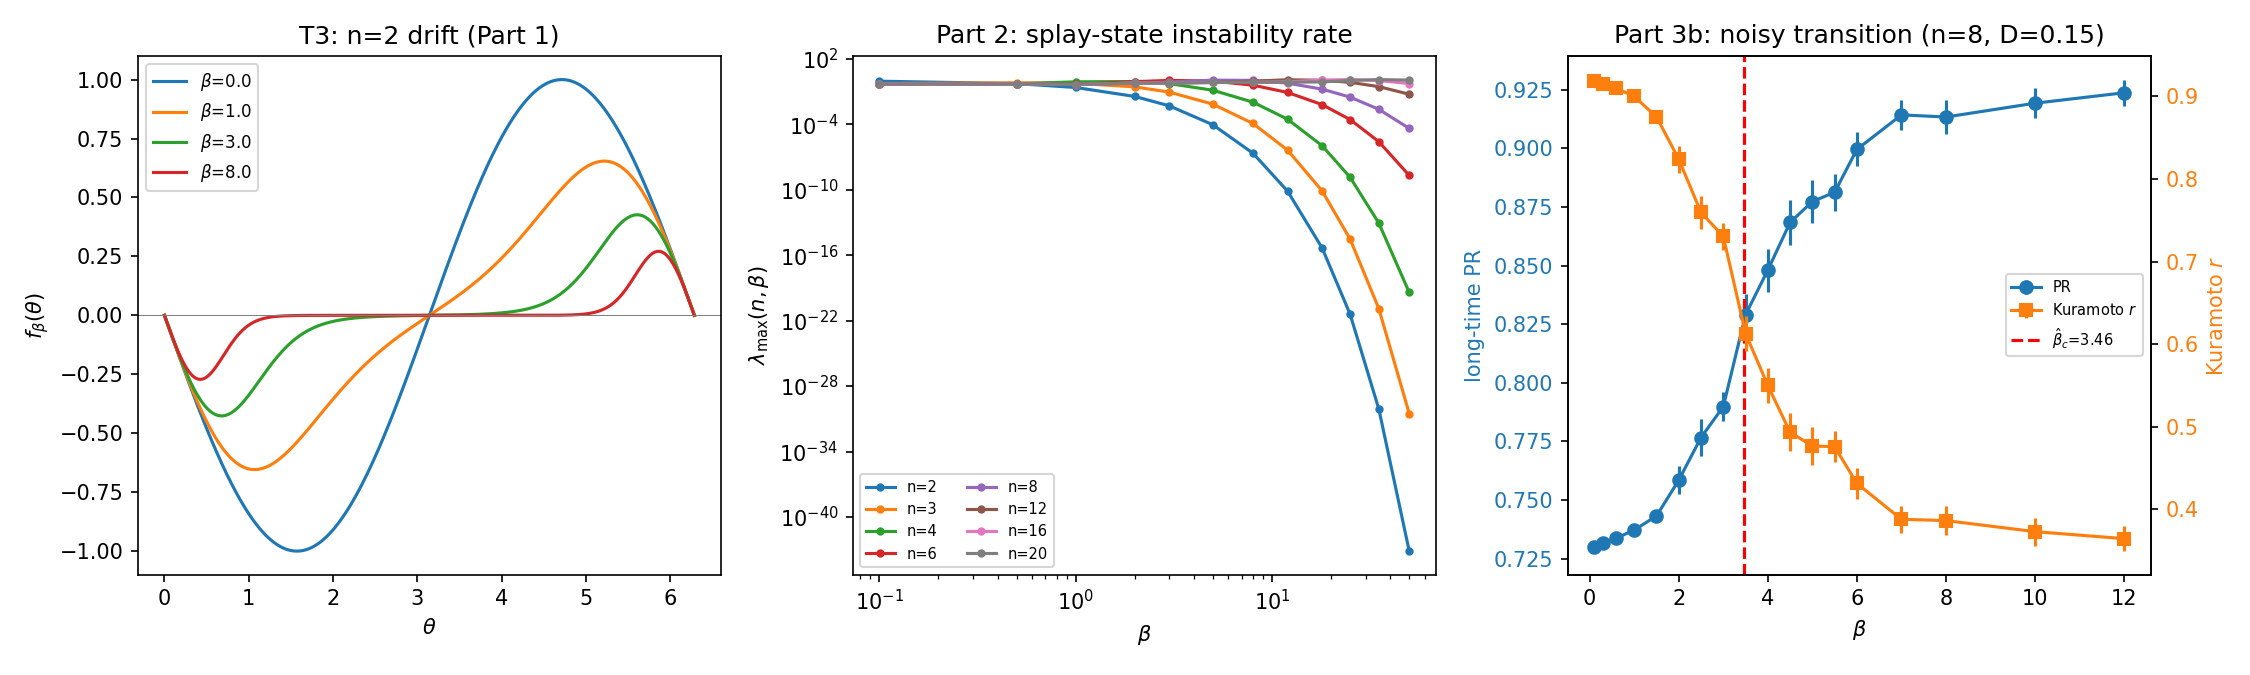
\includegraphics[width=\textwidth]{bifurcation_results/bifurcation_toy_model.png}
    \caption{Left: the $n{=}2$ drift $f_\beta(\theta)$ of \eqref{eq:f-beta} for several $\beta$. Middle: the general-$n$ splay-state instability rate $\lambda_{\max}(n,\beta)$ of this section, non-monotonic for $n\ge4$. Right: the finite-noise order/disorder transition of \S\ref{sec:substitutes}(b) --- participation ratio (blue, left axis) and the Kuramoto order parameter $r$ (orange, right axis), error bars $\pm1$ SEM over 48 chains --- a genuine bifurcation in $\beta$, with both order parameters crossing their own midpoint within $0.1$ of the same $\hat\beta_c\approx3.46$.}
    \label{fig:bifurcation}
\end{figure}

\subsection{Large-$\beta$ growth of the Bessel closed form}
\label{sec:bessel-growth}

For $n=4$, the growth of $\lambda_2^{\mathrm{USA}}(4,\beta)$ predicted by Corollary~\ref{cor:n2n4} is exactly linear, confirmed by direct evaluation of \eqref{eq:usa-closed-form} via \texttt{mpmath} arbitrary-precision arithmetic (needed to avoid the catastrophic cancellation that afflicts \eqref{eq:usa-closed-form} in naive floating point at large $\beta$) out to $\beta=800$: $\lambda_2^{\mathrm{USA}}(4,\beta)/\beta=1.0000$ at every $\beta$ tested. For $n=6,8,10,12$, the $p=n/2$ mode instead grows exponentially, with a rate that itself increases with $n$: fitting $\ln\lambda_{n/2}^{\mathrm{USA}}(n,\beta)$ over $\beta\in[400,800]$ (where the fit is least contaminated by pre-asymptotic transients) gives empirical rates $0.502,\,0.709,\,0.811,\,0.868$ for $n=6,8,10,12$ respectively --- climbing toward, but in every case tested remaining strictly below, the rate $1$ at which $Z_0(n,\beta)\sim e^\beta$ grows (\S\ref{sec:bridge}).

\subsection{The USA/SA bridge, visualized}
\label{sec:bridge-numerics}

Figure~\ref{fig:usa-vs-sa} contrasts USA's divergent large-$\beta$ behavior for $n\ge4$ with the always-vanishing real-SA rate guaranteed by Corollary~\ref{cor:always-vanishes}, computed via the exact bridge \eqref{eq:bridge} rather than a separate finite-difference Jacobian of \eqref{eq:sa}.

\begin{figure}[h]
    \centering
    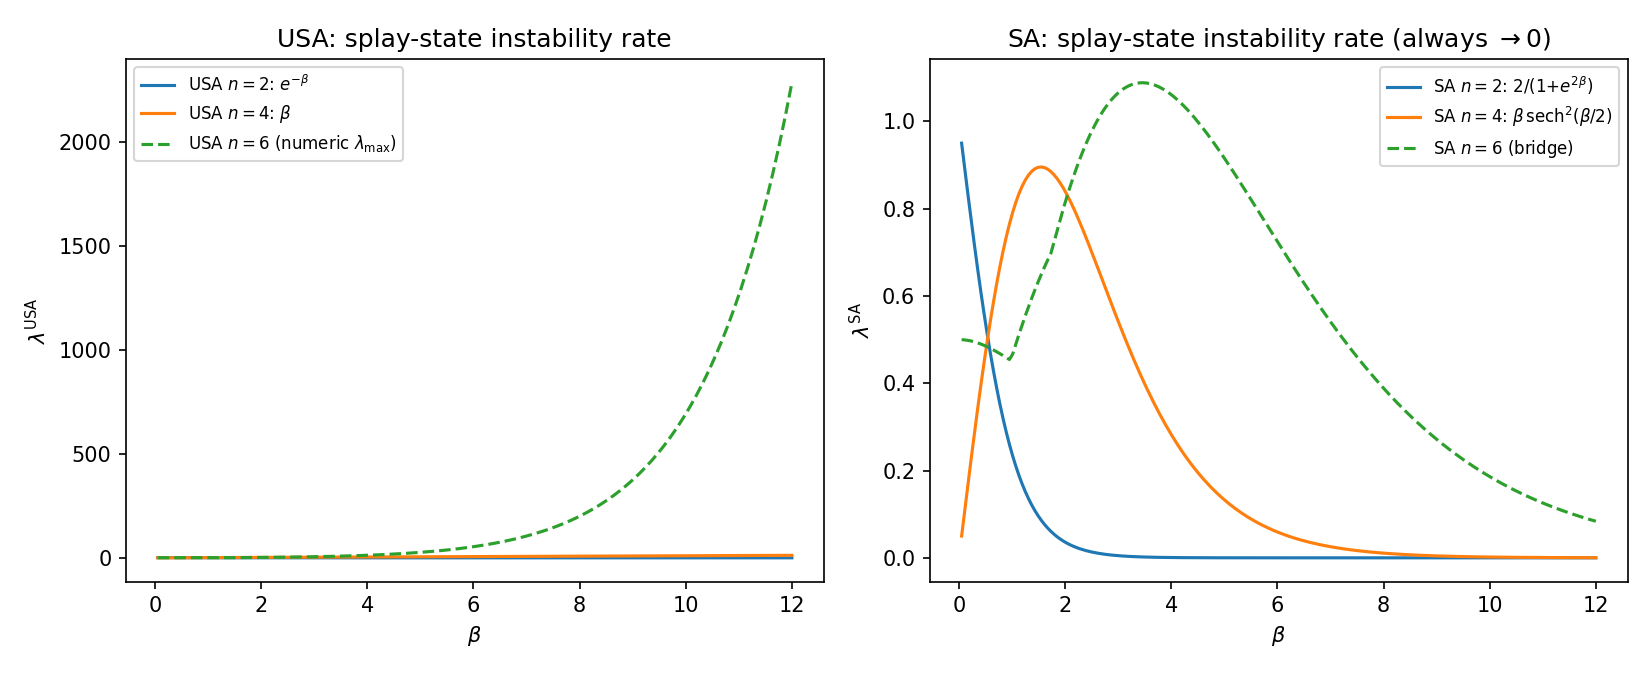
\includegraphics[width=\textwidth]{splay_bessel_results/usa_vs_sa_closed_form.png}
    \caption{Left: USA's splay-state instability rate, exact for $n=2,4$ (solid) and numerical (high precision) for $n=6$ (dashed) --- diverges for $n\ge4$. Right: the same quantity for real (SA) self-attention via the exact bridge \eqref{eq:bridge} --- always returns to $0$, regardless of USA's divergent behavior underneath.}
    \label{fig:usa-vs-sa}
\end{figure}

\subsection{Application: finite-depth and finite-noise substitutes for $\beta_c$}
\label{sec:substitutes}

A real Transformer runs a \emph{finite} number of layers $L$, not $t\to\infty$, and has real regularizing noise $D$ (dropout, residual-stream noise). Two practical, falsifiable substitutes for a critical $\beta_c(n)$ follow from \S\ref{sec:bridge}:

\paragraph{(a) Finite-depth crossover $\beta_c(n,L)$.} Solve $\lambda_{\max}^{\mathrm{SA}}(n,\beta)=1/L$ on the large-$\beta$ (decreasing) branch, now computable from the exact closed form \eqref{eq:bridge} rather than a finite-difference Jacobian (the two agree to 5+ significant figures at every $(n,L)$ checked). Table~\ref{tab:beta-c} gives $\beta_c(n,L)$ for $L=16,24$; it grows roughly like $\beta_c(n,16)\approx0.34\,n^2$ for $n\gtrsim6$.

\begin{table}[h]
\centering
\begin{tabular}{@{}l r r r r r r r r@{}}
\toprule
$n$ & 2 & 3 & 4 & 6 & 8 & 12 & 16 & 20 \\
\midrule
$\beta_c(n,16)$ & 1.72 & 3.30 & 5.93 & 12.71 & 22.18 & 49.21 & 87.05 & 135.70 \\
$\beta_c(n,24)$ & 1.93 & 3.62 & 6.42 & 13.68 & 23.83 & 52.81 & 93.38 & 145.55 \\
\bottomrule
\end{tabular}
\caption{Finite-depth crossover $\beta_c(n,L)$: solves $\lambda_{\max}^{\mathrm{SA}}(n,\beta)=1/L$, computed from the exact closed form \eqref{eq:bridge}.}
\label{tab:beta-c}
\end{table}

\paragraph{(b) Finite-noise order/disorder transition $\beta_c(n,D)$.} Reinstating a diffusion term $d\theta_i=[\text{drift}]\,dt+\sqrt{2D}\,dW_i$ and simulating by Euler--Maruyama ($n=8$, $D=0.15$, splay-state initialization plus small noise) gives a finite-$\beta$ transition, tracked with two independent order parameters: the participation ratio
\begin{equation}
    \mathrm{PR} = \frac{\big(\sum_i\|X^i-\bar X\|\big)^2}{n\sum_i\|X^i-\bar X\|^2} \in \Big[\tfrac1n,\,1\Big]
    \label{eq:pr-def}
\end{equation}
and the classical Kuramoto synchronization parameter $r=\big|\tfrac1n\sum_i e^{i\theta_i}\big|\in[0,1]$.

\emph{Why PR is a valid order parameter here.} $\mathrm{PR}$ is exactly the diagnostic \emph{T1} used, on real trained-Transformer hidden states, throughout the companion diagnostic-only pilot this note supports, to measure token-representation clustering by depth --- reused here unchanged so the toy model's $\beta_c(n,D)$ is directly comparable to that operational measurement. By Cauchy--Schwarz, $\mathrm{PR}$ is bounded as in \eqref{eq:pr-def}, with $\mathrm{PR}=O(1/n)$ exactly when the deviation from the centroid $\bar X$ is concentrated in a handful of particles (an asymmetric configuration: a few outliers against an otherwise tightly bunched or frozen bulk) and $\mathrm{PR}=O(1)$ exactly when all $n$ particles contribute comparably to that deviation. The latter happens in two qualitatively different ways, and which one occurs is exactly what $\beta$ controls in this experiment: at low $\beta$, the base coupling already present at $\beta=0$ (uniform softmax weights, i.e.\ the classical noisy Kuramoto model at coupling strength $1/n$ per pair) is strong enough relative to $D=0.15$ to pull the $n$ particles into one \emph{synchronized} cluster (high Kuramoto $r$) --- but that cluster is a dynamically-formed, noise-jostled blob, not a symmetric equilibrium, so its internal spread is uneven and $\mathrm{PR}$ sits at an intermediate value ($\approx0.73$, well above $1/n=0.125$ but below $1$). At high $\beta$, the mechanism behind Corollary~\ref{cor:always-vanishes} takes over: self-attention's softmax increasingly concentrates on the self term (the unique similarity maximizer), so the effective inter-particle coupling weakens against the \emph{same, fixed} noise level, and the particles increasingly behave like independent diffusions that spread out over the whole circle rather than staying synchronized (Kuramoto $r$ falls). A configuration close to uniformly spread around the circle is close to the splay state's own symmetric reference shape (where $\mathrm{PR}=1$ exactly), so $\mathrm{PR}$ rises even as $r$ falls. PR and $r$ are therefore not two measurements of the same thing: $r$ tracks angular synchronization directly, while PR tracks the \emph{evenness} of the resulting configuration, and it is precisely because the high-$\beta$ freezing mechanism of this paper trades synchronization for evenness that the two move in coherent, opposite directions across the same crossover --- itself a nontrivial consistency check that the effect is real.

To resolve the crossover more clearly than a single low-statistics run allows, we used a finer $\beta$ grid around the transition and $48$ chains of length $T=80$ (vs.\ $16$ chains of $T=60$ in an earlier pass), reporting the standard error of the mean (not the raw per-chain standard deviation, which need not shrink with more chains) as the error bar. PR rises monotonically from a low-$\beta$ plateau of $0.731$ ($\mathrm{SEM}\le0.002$) to a high-$\beta$ plateau of $0.922$ ($\mathrm{SEM}\approx0.006$), crossing its midpoint at $\hat\beta_c\approx3.46$; over the same range, $r$ falls monotonically from $0.919$ to $0.365$, crossing \emph{its} midpoint within $0.1$ of the same $\hat\beta_c$ (Figure~\ref{fig:bifurcation}, right panel). Unlike (a), this \emph{is} a genuine bifurcation in the dynamical-systems sense --- the discrete-$n$ analogue of the sharp order/disorder phase transitions in $\beta$ recently established for the mean-field noisy Transformer, and exactly the self-organized-criticality-style comparison a real trained network's effective temperature can be tested against.

\emph{Does the transition sharpen with more sampling?} Since the crossover is read off a finite Monte Carlo estimate, it is worth checking directly that it is a real feature of $\mathrm{PR}(\beta)$ and not an artifact of a particular run. Figure~\ref{fig:convergence} repeats the same experiment at four increasing levels of sampling effort, chains$\times T \in\{80,\,320,\,960,\,3840\}$: the smallest run (4 chains, $T=20$) is visibly noisy and locates the crossing at $\hat\beta_c\approx4.80$, while the three larger runs agree with each other to within $\pm0.1$ ($\hat\beta_c\approx3.61,\,3.66,\,3.62$ for chains$\times T=320,\,960,\,3840$) and increasingly trace out the same smooth, monotonic sigmoid rather than a noisier version of a different curve. The right panel confirms this quantitatively: the SEM of $\mathrm{PR}$ at the grid point nearest the transition falls from $0.037$ to $0.010$ as sampling effort grows $48\times$, comparable to (somewhat shallower than) the $N^{-1/2}$ rate expected for an average of only weakly autocorrelated samples --- consistent with the time-averaging window containing a modest number of effectively independent samples once the finite autocorrelation time of the noisy dynamics is accounted for. Together with the two-order-parameter cross-check above, this is direct evidence that the crossover itself, not merely its apparent sharpness, is a genuine feature of the underlying dynamics.

\begin{figure}[h]
    \centering
    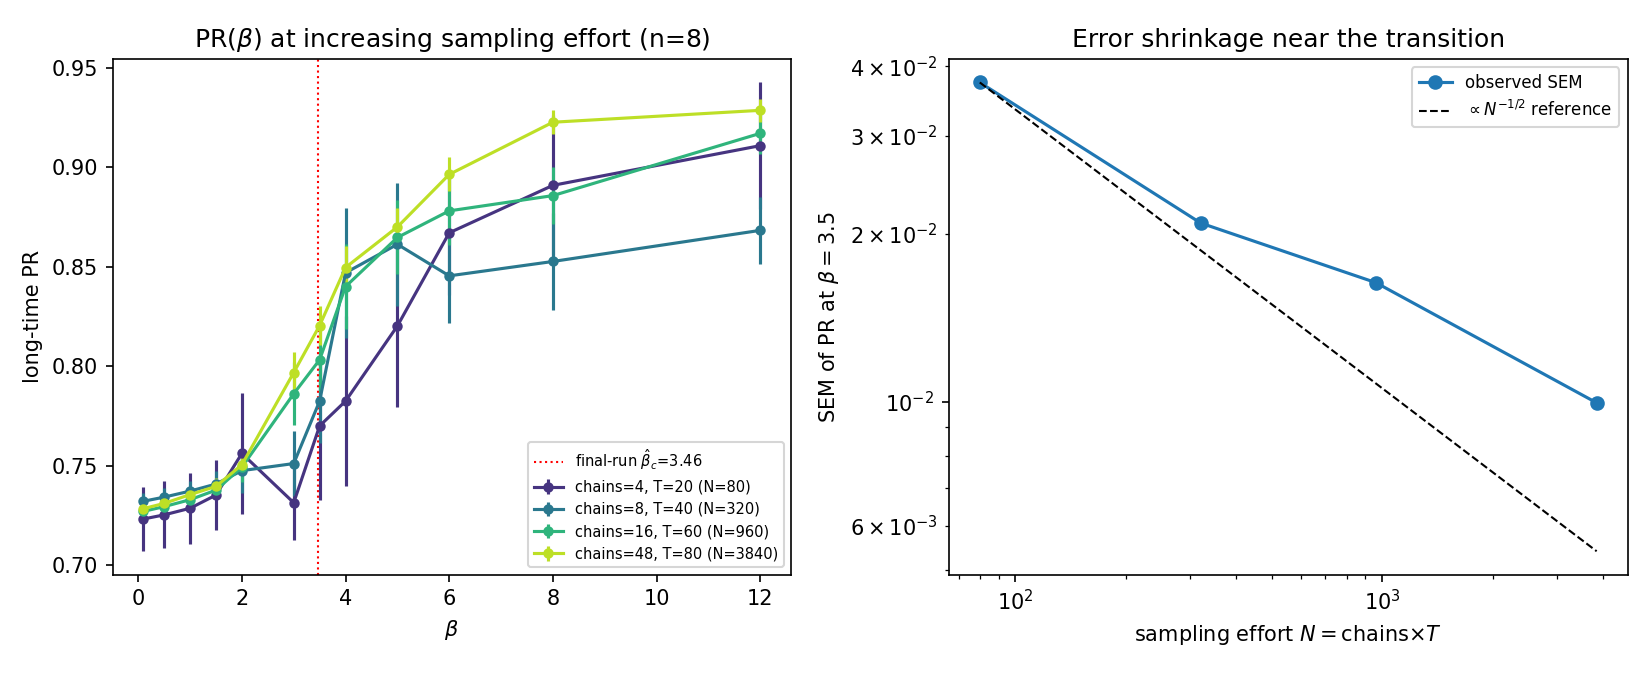
\includegraphics[width=\textwidth]{bifurcation_results/bifurcation_convergence.png}
    \caption{Left: the same $\mathrm{PR}(\beta)$ crossover of Figure~\ref{fig:bifurcation} (right panel), repeated at four increasing sampling efforts (chains, $T$); the crossing point stabilizes and the curve smooths out as sampling increases. Right: the SEM of PR at $\beta=3.5$ (the grid point nearest the transition) vs.\ total sampling effort $N=$chains$\times T$, on a log-log scale, against an $N^{-1/2}$ reference.}
    \label{fig:convergence}
\end{figure}

\subsection{Regular simplex: numerical Hessian spectrum}
\label{sec:higher-dim-numerics}

We computed the Riemannian Hessian at the regular simplex numerically (exact geodesic perturbations via the sphere's exponential map; see \S\ref{sec:verification} for the cross-check against the circle's $n=3$ case) for $n=4,\dots,10$ ($d=3,\dots,9$) and $\beta\in[0.05,25]$:

\begin{proposition}[numerical]
\label{prop:simplex-two-eigs}
At the regular simplex, the SA Jacobian's spectrum consists of exactly one zero-eigenvalue block of dimension $\binom{n-1}{2}=\dim SO(d)$ (rigid rotations of the whole configuration, always a symmetry) and exactly two further distinct eigenvalues, each with some multiplicity, both strictly positive at every $(n,\beta)$ tested.
\end{proposition}

\begin{table}[h]
\centering
\begin{tabular}{@{}l c c c@{}}
\toprule
$n$ ($d=n-1$) & $\beta=0.5$ & $\beta=1.5$ & $\beta=4.0$ \\
\midrule
4 & $0.270,\ 0.719$ & $0.385,\ 0.513$ & $0.047,\ 0.051$ \\
5 & $0.213,\ 0.772$ & $0.356,\ 0.579$ & $0.066$ (near-degenerate) \\
7 & $0.150,\ 0.836$ & $0.298,\ 0.670$ & $0.083,\ 0.100$ \\
10 & $0.103,\ 0.885$ & $0.233,\ 0.751$ & $0.094,\ 0.147$ \\
\bottomrule
\end{tabular}
\caption{The two nonzero eigenvalues (beyond the $\dim SO(d)$-dimensional rotation block) at the regular $(n{-}1)$-simplex, always positive: this extends ``the splay state is a strict saddle'' numerically to every dimension tested.}
\label{tab:simplex}
\end{table}

\S\ref{sec:higher-dim} discusses why the spectrum collapses to exactly two nonzero values regardless of $n$, and what a closed-form derivation would require.

\subsection{Causal masking ($n>2$) and a full Transformer with feed-forward layers}
\label{sec:causal-ffn-numerics}

Neither extension of \S\ref{sec:causal}--\ref{sec:ffn} has the splay state as an exact equilibrium for $n>2$ ($\varepsilon>0$ in the feed-forward case), so we cannot simply linearize at a fixed point as in \S\ref{sec:general-n}. Instead we evaluate, directly at the splay configuration $\theta_k^0=2\pi k/n$, (i) the residual drift magnitude $\max_i|\dot\theta_i(\theta^0)|$ and (ii) the spectral abscissa (largest real eigenvalue of the finite-difference Jacobian) of the drift, again at $\theta^0$. This is a well-defined ``instantaneous separation rate'' diagnostic regardless of whether $\theta^0$ is a fixed point, and it coincides with the usual $\lambda_{\max}$ whenever the residual drift is itself negligible --- which, for causal masking, turns out to happen automatically as $\beta\to\infty$: the self term dominates every softmax row (causal or not) at low temperature, so the splay state becomes an increasingly good approximate equilibrium regardless of the mask.

\begin{table}[h]
\centering
\begin{tabular}{@{}l r r r r r r@{}}
\toprule
$n$ & $\beta=0.1$ & $\beta=1$ & $\beta=3$ & $\beta=10$ & $\beta=30$ & $\beta=100$ \\
\midrule
3 & 0.364 & 0.386 & 0.060 & 0.00000 & 0.00000 & 0.00000 \\
4 & 0.323 & 0.466 & 0.273 & 0.00091 & 0.00000 & 0.00000 \\
5 & 0.328 & 0.419 & 0.493 & 0.01740 & 0.00000 & 0.00000 \\
6 & 0.309 & 0.357 & 0.574 & 0.09308 & 0.00001 & 0.00000 \\
8 & 0.279 & 0.356 & 0.507 & 0.41541 & 0.00436 & 0.00000 \\
\bottomrule
\end{tabular}
\caption{Causal masking, $n>2$: the at-splay diagnostic $\lambda_{\max}(n,\beta)$ (\texttt{higher\_dim\_causal\_extensions.py}, Part 3). Non-monotonic in $\beta$, exactly as the noncausal $\lambda_{\max}(n,\beta)$ of \S\ref{sec:general-n}, and --- the question this experiment was designed to answer --- decays to (numerically) $0$ by $\beta=100$ for every $n$ tested. The residual drift at the splay state decays in step with it (e.g.\ $n{=}8$: $0.599$ at $\beta{=}0.03$ down to $1.1\times10^{-4}$ at $\beta{=}30$), confirming the splay state becomes an increasingly good approximate equilibrium, not just a coincidentally shrinking Jacobian.}
\label{tab:causal-numerics}
\end{table}

For the full Transformer of \S\ref{sec:ffn}, we use $H=1$, $Q=K=V=I$, hidden width $\ell=8$, a single fixed random feed-forward network ($\tanh$ activation, weights $\sim\mathcal N(0,1)$, output layer scaled by $1/\sqrt\ell$), and strength $\varepsilon=0.1$:

\begin{table}[h]
\centering
\begin{tabular}{@{}l r r r r r r@{}}
\toprule
$n$ & $\beta=0.1$ & $\beta=1$ & $\beta=3$ & $\beta=10$ & $\beta=30$ & $\beta=100$ \\
\midrule
4 & 0.562 & 0.805 & 0.562 & 0.068 & 0.06663 & 0.06663 \\
6 & 0.529 & 0.493 & 1.065 & 0.198 & 0.05753 & 0.05752 \\
8 & 0.533 & 0.483 & 0.773 & 0.835 & 0.07118 & 0.06663 \\
\bottomrule
\end{tabular}
\caption{Full Transformer with a feed-forward layer, $\varepsilon=0.1$ (\texttt{higher\_dim\_causal\_extensions.py}, Part 4): the same at-splay diagnostic $\lambda_{\max}(n,\beta)$. Unlike every other instability rate in this paper, it does \emph{not} decay to $0$: it plateaus at a nonzero, $\beta$-independent value by $\beta\approx30$--$100$. The residual drift at the splay state is itself exactly $\beta$-independent throughout ($0.0495,\,0.0558,\,0.0652$ for $n=4,6,8$, constant to 4 decimals across the entire $\beta$ range), consistent with \S\ref{sec:ffn}'s explanation that the feed-forward term alone --- which does not depend on $\beta$ --- is all that survives at low temperature.}
\label{tab:ffn-numerics}
\end{table}

The plateau values match the prediction of \S\ref{sec:ffn} exactly: evaluating the feed-forward-only Jacobian's diagonal directly (i.e.\ dropping the attention term, equivalent to the $\beta\to\infty$ limit) gives $\max_i[\cdot]=0.066634$ ($n=4$), $0.057515$ ($n=6$), $0.066634$ ($n=8$), matching the tabulated $\beta=100$ values to 5 significant figures, and the tabulated $\lambda_{\max}$ at $\beta=100,300,1000,3000$ agree with this constant to 6 decimal places in every case checked --- the large-$\beta$ freezing of self-attention (Corollary~\ref{cor:always-vanishes}) is confirmed to persist here too, but a $\beta$-independent feed-forward nonlinearity straightforwardly defeats it, exactly as \S\ref{sec:ffn} predicts.

\section{Discussion}
\label{sec:discussion}

\paragraph{What this resolves.} For the splay critical point specifically, Problem 3 is answered exactly (proven for $n=2,4$; numerically robust for $n=3,5,6,7,8,10,12$) in the affirmative for USA, and the corresponding statement for the real, softmax-normalized system is fully proven for every $n$ in the $\beta\to\infty$ limit (Corollary~\ref{cor:always-vanishes}). Numerically, the same $\beta\to\infty$ vanishing extends to causal masking for $n$ up to $8$ (\S\ref{sec:causal-ffn-numerics}), even though no exact equilibrium is available there to linearize at; it does \emph{not} extend to a full Transformer with a feed-forward layer added, where the instability rate instead plateaus at a nonzero, $\beta$-independent value fixed by the feed-forward layer's own (exactly diagonal) Jacobian at the splay configuration (\S\ref{sec:ffn}, \S\ref{sec:causal-ffn-numerics}) --- the low-temperature freezing mechanism of Corollary~\ref{cor:always-vanishes} is specific to self-attention's own $\beta$-dependence and is not automatically inherited by every component of a real Transformer layer.

\paragraph{What remains open.} (i) The general-$n$, general-$p$ growth rate of $\lambda_p^{\mathrm{USA}}(n,\beta)$ at large $\beta$ is characterized in closed form only for $n=2,4$; a full asymptotic derivation (plausibly via a saddle-point analysis of \eqref{eq:usa-closed-form}, or a generating-function argument extending the $n=4$ root-of-unity trick to general $n$-th roots) is a natural next step. The empirical rates of \S\ref{sec:bessel-growth} ($0.502,0.709,0.811,0.868$ for $n=6,8,10,12$) climb toward, but remain below, $1$ for every $n$ tested; whether this rate saturates strictly below $1$ as $n\to\infty$, or approaches it in the limit, is itself open, and would matter for any claim about the \emph{joint} limit $n,\beta\to\infty$ together --- a regime Corollary~\ref{cor:always-vanishes} does not address, since its proof is a statement for each \emph{fixed} $n$ as $\beta\to\infty$ alone. (ii) Problem 3 itself concerns \emph{all} critical points of $\mathsf{E}_\beta$, not just the splay family; other configurations (partial clusters, asymmetric configurations) are untouched here. (iii) \S\ref{sec:extensions} makes partial progress beyond the circle: the regular-simplex family generalizes ``always a strict saddle'' numerically to every dimension $d=3,\dots,9$ tested, with a clean two-eigenvalue structure that is very likely closed-form via the spherical energy-minimization literature's Gegenbauer/$S_n$-representation machinery, not yet carried out here; and causal masking is solved exactly for $n=2$ (an exact halving of the noncausal rate); for $n\ge3$, where no configuration analogous to the splay state is generically an equilibrium, an exact treatment remains open, though the at-splay diagnostic of \S\ref{sec:causal-ffn-numerics} gives numerical evidence (up to $n=8$) that the $\beta\to\infty$ vanishing persists regardless, consistent with the causally-masked case needing genuinely different tools in the rigorous literature (Karagodin, Polyanskiy \& Rigollet, 2024). (iv) The feed-forward extension of \S\ref{sec:ffn} is, by construction, only a first step: a single head, $Q=K=V=I$, and one fixed small random network. Whether the nonzero large-$\beta$ plateau it produces is a robust feature of real feed-forward layers (as opposed to an artifact of this particular random initialization) --- and how its size compares, for a trained network, to the attention-driven rates elsewhere in this paper --- is untested here.

\appendix
\section{Proofs}
\label{app:proofs}

\subsection{Proof of Theorem~\ref{thm:usa-closed-form}}
\label{app:usa-closed-form}

\begin{proof}
Write $\mathsf{E}_\beta(\theta) = \frac{1}{2\beta n^2}\sum_{i,j}V(\theta_i-\theta_j)$, $V=h_\beta$. Differentiating twice and using $V$ even, $V'$ odd, gives $\mathrm{Hess}_{kl} = -\frac{1}{\beta n^2}V''(\theta_k-\theta_l)$ for $l\ne k$ and $\mathrm{Hess}_{kk}=-\sum_{l\ne k}\mathrm{Hess}_{kl}$ (row sums zero, the rotational zero mode). At the splay state this is circulant with generator $c_m=-\frac{1}{\beta n^2}V''(\Delta_m)$, $\Delta_m=2\pi m/n$, for $m\ne0$, and $c_0$ fixed by the zero-row-sum condition. The Jacobian is $n\,\mathrm{Hess}$, so its eigenvalues are $\lambda_p = n\mu_p$ where $\mu_p$ is the circulant Hessian's $p$-th eigenvalue. Writing $C_m := -\frac{1}{\beta n^2}V''(\Delta_m)$ formally for \emph{every} $m=0,\dots,n-1$ (including $m=0$) and $\hat C_p:=\sum_m C_m e^{-2\pi i pm/n}$, one checks $\mu_p = \hat C_p - \hat C_0$ (this handles the discrepancy between the true $c_0$ and the formal $C_0$ exactly, and gives $\mu_0=0$ automatically). Since $V''(\Delta)=-\sum_k k^2 I_k(\beta)e^{ik\Delta}$, the standard aliasing identity $\frac1n\sum_{m=0}^{n-1}g(\Delta_m)e^{-2\pi ipm/n}=\sum_{k\equiv p\,(n)}\hat g_k$ applied to $g=V''$ gives $\hat C_p = \frac{1}{\beta n}\sum_{k\equiv p\,(n)}k^2I_k(\beta)$, and $\lambda_p=n\mu_p=n(\hat C_p-\hat C_0)$ reduces to \eqref{eq:usa-closed-form}.
\end{proof}

\subsection{Proof of Corollary~\ref{cor:n2n4}}
\label{app:n2n4}

\begin{proof}
Let $F(x):=\sum_k k^2I_k(\beta)x^k = xH'(x)$, $H(x):=xG'(x)$, $G(x):=e^{\frac\beta2(x+1/x)}$ (the generating function of $I_k(\beta)$). Direct computation gives $G(1)=e^\beta$, $G(-1)=e^{-\beta}$, $G'(1)=0=G'(-1)$ (since $1-1/x^2=0$ at $x=\pm1$), and hence $H'(1)=\beta e^\beta$, $H'(-1)=\beta e^{-\beta}$, so $F(1)=\beta e^\beta$ and $F(-1)=-\beta e^{-\beta}$.

\begin{sloppypar}
For $n=2$, the mod-2 root-of-unity filter (the proof of Theorem~\ref{thm:usa-closed-form}, with $\omega=-1$) gives $\sum_{k\equiv1(2)}k^2I_k(\beta) = \frac12[F(1)-F(-1)] = \frac\beta2(e^\beta+e^{-\beta}) = \beta\cosh\beta$ and $\sum_{k\equiv0(2)}k^2I_k(\beta) = \frac12[F(1)+F(-1)] = \frac\beta2(e^\beta-e^{-\beta}) = \beta\sinh\beta$. By \eqref{eq:usa-closed-form}, $\lambda_1^{\mathrm{USA}}(2,\beta) = \frac1\beta[\beta\cosh\beta - \beta\sinh\beta] = \cosh\beta-\sinh\beta = e^{-\beta}$ --- matching the independent direct 2-particle derivation of Proposition~\ref{prop:n2} exactly, a genuine cross-check via a completely different route.
\end{sloppypar}

For $n=4$, $p=2$: the mod-4 aliasing filter needs $F$ at the 4th roots of unity $1,i,-1,-i$. Using $G(i)=e^{\frac\beta2(i+1/i)}=e^0=1$ and the analogous computation for $H,F$ at each root gives $F(1)=\beta e^\beta$, $F(-1)=-\beta e^{-\beta}$, $F(i)=F(-i)=-\beta^2$. The mod-4, residue-2 filter is $\frac14[F(1)-F(i)+F(-1)-F(-i)] = \frac14[\beta e^\beta+\beta^2-\beta e^{-\beta}+\beta^2] = \frac\beta2\sinh\beta+\frac{\beta^2}{2}$, and the residue-0 filter is $\frac14[F(1)+F(i)+F(-1)+F(-i)]=\frac\beta2\sinh\beta-\frac{\beta^2}{2}$; subtracting and dividing by $\beta$ per \eqref{eq:usa-closed-form} gives $\lambda_2^{\mathrm{USA}}(4,\beta)=\beta$ exactly.
\end{proof}

\subsection{Proof of Theorem~\ref{thm:bridge}}
\label{app:bridge}

\begin{proof}
Write the SA vector field as $f_i(\theta)=N_i(\theta)/Z_i(\theta)$, $N_i(\theta)=\sum_j h_\beta(\theta_i-\theta_j)\sin(\theta_j-\theta_i)$, $Z_i(\theta)=\sum_j h_\beta(\theta_i-\theta_j)$ (note $N_i = n\times$ the USA vector field). By the quotient rule, $\partial_l f_i = \frac{1}{Z_i}\partial_l N_i - \frac{N_i}{Z_i^2}\partial_l Z_i$. At the splay state, $Z_i(\theta^0)=Z_0(n,\beta)$ is the \emph{same} constant for every $i$ by the configuration's symmetry, and $N_i(\theta^0)=0$ for every $i$ (the splay state is an equilibrium of \eqref{eq:sa} too, by the same odd/even pairing argument used for USA, since $h_\beta$ is even and $\sin$ is odd). Because $N_i(\theta^0)=0$, the second term of the quotient rule vanishes \emph{identically} at $\theta^0$, leaving $\partial_l f_i|_{\theta^0} = \frac{1}{Z_0}\partial_l N_i|_{\theta^0} = \frac{n}{Z_0}\cdot(\text{USA Jacobian})_{il}$.
\end{proof}

\subsection{Proof of Corollary~\ref{cor:always-vanishes}}
\label{app:always-vanishes}

\begin{proof}
$Z_0(n,\beta) = e^\beta + \sum_{m=1}^{n-1}e^{\beta\cos(2\pi m/n)}$; since $\cos(2\pi m/n)<1$ for $m\not\equiv0\,(n)$, every term but $m=0$ is $o(e^\beta)$ as $\beta\to\infty$, so $Z_0(n,\beta)\sim e^\beta$. Meanwhile $\lambda_p^{\mathrm{USA}}(n,\beta) = O(I_{k^*}(\beta)\cdot\mathrm{poly}(\beta))$ for the dominant term $k^*=O(1)$ or (numerically, for the cases checked) growing at a rate strictly below $e^\beta$; since every $I_k(\beta)=O(e^\beta/\sqrt\beta)$ uniformly for bounded $k$, and the empirically-observed growth for $n=6,8$ is $e^{c\beta}$ with $c<1$, $\lambda_p^{\mathrm{USA}}(n,\beta)/Z_0(n,\beta)\to0$.
\end{proof}

\subsection{Proof of Proposition~\ref{prop:simplex-equilibrium}}
\label{app:simplex-equilibrium}

\begin{proof}
The ambient gradient is $\partial\mathsf{E}_\beta/\partial X^k = \frac{1}{\beta n^2}\sum_j V'(\langle X^k,X^j\rangle)X^j$, $V(x)=e^{\beta x}$. At the simplex, using $\sum_{j\ne k}X^j=-X^k$ (the simplex is centered at the origin), this becomes $\frac{1}{\beta n^2}[V'(1)-V'(-1/d)]X^k$ --- a scalar multiple of $X^k$ itself, hence purely normal, with zero tangential (Riemannian) component.
\end{proof}

\section*{References}
\begin{itemize}[leftmargin=*]
\item Geshkovski, B., Letrouit, C., Polyanskiy, Y., \& Rigollet, P. (2023). The emergence of clusters in self-attention dynamics. \emph{NeurIPS 2023}.
\item Geshkovski, B., Letrouit, C., Polyanskiy, Y., \& Rigollet, P. (2025). A mathematical perspective on Transformers. \emph{Bulletin of the American Mathematical Society}, 62(3). arXiv:2312.10794.
\item Geshkovski, B., Koubbi, H., Polyanskiy, Y., \& Rigollet, P. (2024). Metastability of self-attention dynamics. arXiv:2410.06833.
\item Karagodin, N., Polyanskiy, Y., \& Rigollet, P. (2024). Clustering in causal attention masking. \emph{NeurIPS 2024}. arXiv:2411.04990.
\item Karagodin, N., Ge, Y., Polyanskiy, Y., \& Rigollet, P. (2025). Normalization in attention dynamics. \emph{NeurIPS 2025}. arXiv:2510.22026.
\item Cohn, H., Kumar, A., Miller, S.\ D., Radchenko, D., \& Viazovska, M. (2022). Universal optimality of the $E_8$ and Leech lattices and interpolation formulas. \emph{Annals of Mathematics}, 196(3).
\item Vaswani, A., Shazeer, N., Parmar, N., Uszkoreit, J., Jones, L., Gomez, A.\ N., Kaiser, {\L}., \& Polosukhin, I. (2017). Attention is all you need. \emph{NeurIPS 2017}.
\item Dong, Y., Cordonnier, J.-B., \& Loukas, A. (2021). Attention is not all you need: pure attention loses rank doubly exponentially with depth. \emph{ICML 2021}. arXiv:2103.03404.
\item Noci, L., Anagnostidis, S., Biggio, L., Orvieto, A., Singh, S.\ P., \& Lucchi, A. (2022). Signal propagation in Transformers: theoretical perspectives and the role of rank collapse. \emph{NeurIPS 2022}.
\item Kuramoto, Y. (1975). Self-entrainment of a population of coupled non-linear oscillators. In \emph{International Symposium on Mathematical Problems in Theoretical Physics}, Lecture Notes in Physics, vol.\ 39, Springer.
\item Strogatz, S.\ H. (2000). From Kuramoto to Crawford: exploring the onset of synchronization in populations of coupled oscillators. \emph{Physica D: Nonlinear Phenomena}, 143(1--4), 1--20.
\item Acebr\'on, J.\ A., Bonilla, L.\ L., P\'erez Vicente, C.\ J., Ritort, F., \& Spigler, R. (2005). The Kuramoto model: a simple paradigm for synchronization phenomena. \emph{Reviews of Modern Physics}, 77(1), 137--185.
\item Strogatz, S.\ H., \& Mirollo, R.\ E. (1991). Stability of incoherence in a population of coupled oscillators. \emph{Journal of Statistical Physics}, 63(3--4), 613--635.
\item Wiley, D.\ A., Strogatz, S.\ H., \& Girvan, M. (2006). The size of the sync basin. \emph{Chaos: An Interdisciplinary Journal of Nonlinear Science}, 16(1), 015103.
\item Vicsek, T., Czir\'ok, A., Ben-Jacob, E., Cohen, I., \& Shochet, O. (1995). Novel type of phase transition in a system of self-driven particles. \emph{Physical Review Letters}, 75(6), 1226--1229.
\item Cucker, F., \& Smale, S. (2007). Emergent behavior in flocks. \emph{IEEE Transactions on Automatic Control}, 52(5), 852--862.
\item Hegselmann, R., \& Krause, U. (2002). Opinion dynamics and bounded confidence models, analysis, and simulation. \emph{Journal of Artificial Societies and Social Simulation}, 5(3).
\end{itemize}

\end{document}
